\documentclass[11pt,a4paper,dvipdfmx]{article}
%\documentclass[autodetect-engine,dvipdfmx-if-dvi,ja=standard]{bxjsarticle}

\usepackage{ascmac}
\usepackage[utf8]{inputenc}
\usepackage{lmodern}
\usepackage[T1]{fontenc}
\usepackage[noBBpl]{mathpazo}
%\linespread{1.05}
\usepackage{mathtools, amsmath, amssymb, amsthm}
\usepackage{amsfonts}
\usepackage{braket}
%\usepackage{amssymb}
\usepackage{url}
\usepackage{bbm}

%% citation
\usepackage[longnamesfirst]{natbib}

%
%\theoremstyle{plain}
%\newtheorem{thm}{Thm.}[section]
%\newtheorem{lem}{Lem.}[section]
%\newtheorem{cor}{Cor.}[section]
%\newtheorem{prop}{Prop.}[section]
%\newtheorem{df}{Def.}[section]
%\newtheorem{eg}{e.g.}[section]
%\newtheorem{rem}{Rem.}[section]
%\theoremstyle{plain}
\newtheorem{thm}{Thm.}
\newtheorem{lem}{Lem.}
\newtheorem{cor}{Cor.}
\newtheorem{prop}{Prop.}
\newtheorem{df}{Def.}
\newtheorem{eg}{e.g.}
\newtheorem{rem}{Rem.}
%

\usepackage{listings}
\lstset{%
language={python},%
basicstyle={\ttfamily\footnotesize},%ソースコードの文字を小さくする
frame={single},
commentstyle={\footnotesize\itshape},%コメントアウトの文字を小さくする
breaklines=true,%行が長くなったときの改行。trueの場合は改行する。
numbers=left,%行番号を左に書く。消す場合はnone。
xrightmargin=3zw,%左の空白の大きさ
xleftmargin=3zw,%右の空白の大きさ
stepnumber=1,%行番号を1から始める場合こうする(たぶん)
numbersep=1zw,%行番号と本文の間隔。
}

%\usepackage[dvipdfmx]{graphicx}
%% color packageとdvipdfmxは相性が悪いらしい
%% https://qiita.com/zr_tex8r/items/442b75b452b11bee8049
\usepackage{graphicx}


\usepackage[left=2cm,right=2cm,top=2cm,bottom=2cm]{geometry} %This changes the margins.
\usepackage{float}
%\author{Kyohei Okumura}
\global\long\def\T#1{#1^{\top}}

\newcommand{\id}{\textnormal{id}}
\newcommand{\R}{\mathbb{R}}
\newcommand{\N}{\mathbb{N}}
\newcommand{\Q}{\mathbb{Q}}
\newcommand{\Z}{\mathbb{Z}}
\newcommand{\C}{\mathbb{C}}
\newcommand{\mF}{\mathcal{F}}
\newcommand{\mG}{\mathcal{G}}
\newcommand{\mA}{\mathcal{A}}
\newcommand{\mB}{\mathcal{B}}
\newcommand{\mC}{\mathcal{C}}
\newcommand{\mD}{\mathcal{D}}
\newcommand{\mE}{\mathcal{E}}
\newcommand{\mL}{\mathcal{L}}
\newcommand{\mM}{\mathcal{M}}
\newcommand{\mN}{\mathcal{N}}
\newcommand{\mO}{\mathcal{O}}
\newcommand{\mP}{\mathcal{P}}
\newcommand{\mS}{\mathcal{S}}
\newcommand{\mT}{\mathcal{T}}
\newcommand{\mV}{\mathcal{V}}
\newcommand{\mW}{\mathcal{W}}
\newcommand{\mX}{\mathcal{X}}
\newcommand{\mZ}{\mathcal{Z}}
\renewcommand{\Re}{\mathrm{Re}}
\renewcommand{\hat}{\widehat}
\renewcommand{\tilde}{\widetilde}
\renewcommand{\bar}{\overline}
\renewcommand{\epsilon}{\varepsilon}
% \renewcommand{\span}{\mathrm{span}}
\newcommand{\defi}{\stackrel{\Delta}{\Longleftrightarrow}}
\newcommand{\equi}{\Longleftrightarrow}
\newcommand{\s}{\succsim}
\newcommand{\p}{\precsim}
\newcommand{\join}{\vee}
\newcommand{\meet}{\wedge}
%\newcommand{\1}{\mbox{1}\hspace{-0.25em}\mbox{l}}
\newcommand{\1}{\mathbbm{1}}
\newcommand{\E}{\mathbbm{E}}

\DeclareMathOperator{\Var}{Var}
\DeclareMathOperator{\Cov}{Cov}
\DeclareMathOperator{\sgn}{sgn}
\DeclareMathOperator{\Card}{Card}
\DeclareMathOperator{\supp}{supp}
\DeclareMathOperator{\Log}{Log}
\DeclareMathOperator{\spn}{span}

\newcommand{\indep}{\mathop{\perp\!\!\!\!\perp}}

\usepackage{color}
\newcommand{\kcomment}[1]{{\textcolor{blue}{#1}}}
\newcommand{\ocomment}[1]{{\textcolor{red}{#1}}}

%%%%%%%%%%%%%%%%%%%%%%%%%%%%%%%%%%%%%%%%%%%%%%%

\begin{document}
\title{Notes on Dynamic Delegation}
\author{Kyohei Okumura{\footnote{E-mail: kyohei.okumura@gmail.com}
}}
\date{\today}
\maketitle

\section*{Motivation}
\begin{itemize}
	\item Dynamic delegation to multiple heterogeneously specialized agents
	\item one principal v.s. many agents. Misalignment of interests.
	\begin{itemize}
		\item manager v.s. workers
		\item head quarters(overall profits) v.s. division managers(their own division's profits)
		\item A military v.s. elite units (a prestigious operation)
	\end{itemize}
	\item 各期に一つtaskが降ってくる.毎期最も適している人に割り当てたい.
	\item Monetary transfer, commitment to future allocation decisionsが不可能な状況下でのdynamic mechanism design.
	\begin{itemize}
		\item monetary transferによる動機付けが難しいのはorganizational decision makingではよくありそう?
		\item \ocomment{commitmentが難しいってどういう状況?この仮定は重要なの?}
	\end{itemize}
\end{itemize}

\section*{Model}
\begin{itemize}
	\item Players $i \in \{0,1,2\}$. principal: 0, agents: 1,2
	\item $\omega_t \in \{A, B\}$: the type of period-$t$ job, observable from everyone.
	\item $\theta_{it} \in \{\alpha, \beta\}$: agent $i$'s type in period $t$, private info.
	\item $\phi^i \in [0,1]$: $i$'s specialization, common knowledge.
	\begin{itemize}
		\item $\Pr(\theta_{it} = \alpha) = \phi^i$, independent across periods and agents.
		\item $\phi^i$の値が大きいほど,task $A$に向いている.
		\item Assume for simplicity that $\phi^1 := \phi, \ \phi^2 := 1 - \phi \quad (\phi \in [1/2,1))$.
	\end{itemize}
	\item $y_t \in \{0,S,F\}$: outcome. $y_t=0$は,その気に誰にもtaskを割り振らなかったことを意味する.$S, F$はそれぞれ,successとfailureを表す.
	\item $\Pr(y_t = S \mid (\theta_{it}, \omega_t) \in \{(\alpha, A), (\beta, B) \}, \text{$i$ is assigned}) = \bar{\mu}$
	\item $\Pr(y_t = S \mid (\theta_{it}, \omega_t) \in \{(\alpha, B), (\beta, A) \}, \text{$i$ is assigned}) = \underline{\mu}$, $(\underline{\mu} < \bar{\mu})$
	
	\begin{figure}[H]
	  \centering
	    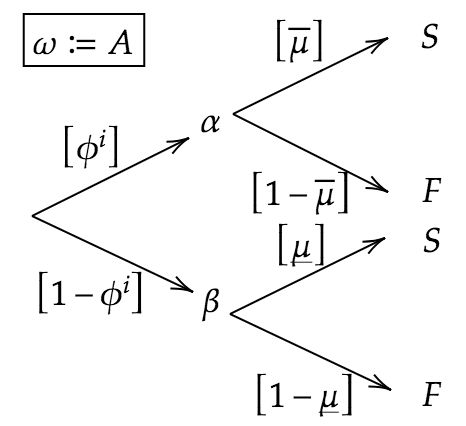
\includegraphics[height=5cm]{image/adverse.png}
	\end{figure}
	\item Repeated games model.
	\item Each period-$t$ stage game proceeds as follows:
	\begin{enumerate}
		\item $\omega_t \in \{A,B\}$ realizes with equal probability. Everyone observes the value of $\omega_t$. 
		\item Each agent $i$ send a message $m_{it} \in \{0,1\}$ to the principal simultaneously.
		\item The principal allocate the task to one of the agents $j_t = i \in \{1,2\}$, or throw it away ($j_t = 0$).
		\item Whether the agent succeeds or not, $y_t$, is observed. Payoff realizes.
		\item (Public Randomization) 
	\end{enumerate}
	\item \ocomment{Adverse selection + Imperfect monitering}
	\item period-$t$ history: $((m_{1t}, m_{2t}), \omega_t, j_t, y_t)$
	\begin{itemize}
		\item $m_{it}$: the message that the agent send in period $t$
		\item $\omega_t \in \{A, B\}$: the type of period-$t$ task
		\item $y_t \in \{0, S, F\}$: success or failure. 
		\item $j_t \in \{0,1,2\}$: who is assigned
		\item $j_t = 0$は,どちらのagentにも割り振らないことを表す.(その場合,全員の利得0.)
		\item \ocomment{$j_t = 0$ (どちらのagentにも振らない)をモデルに入れる必要があるか?元論文では入れているが,不必要なようにも思える.要検討.(feasible payoffにも影響?)}
	\end{itemize}
	\item public history: $h^t := ((m_{1\tau}, m_{2\tau}), \omega_\tau, j_\tau, y_\tau)_{\tau=1}^{t-1}$
	\item Utility functions:
	\begin{itemize}
		\item $\displaystyle{U_0 := (1 - \delta) \sum_t \delta^t \1_{\{y_t = S\}} }, \quad 
		\displaystyle{U_i := (1 - \delta) \sum_t \delta^t  \pi \1_{\{j_t = i \}}\1_{\{y_t = S\}} \ (i \in \{1,2\})}$
		\item principalは,仕事が成功すると利得1.agentは,仕事が自分に振られた上で仕事に成功すると利得$\pi$をその期に得る.
		\item myopicallyには,「俺が俺が」といって仕事を振られた方がagentとしては得.
	\end{itemize}
	\item 均衡概念としては,ex-post public perfect equilibrium(XPPE) を考える.
	\begin{itemize}
		\item public perfect equilibrium: public strategy(public historyにのみ依存した戦略)による均衡.
		\item $\sigma: \text{PPE} \defi \forall i; \sigma_i \text{ is public}, \ \forall t \forall h^{t-1}; \sigma: \text{ NE from that time on.}$
		\item ``ex-post'': 各agentは,その期の他のプレイヤーのタイプに関するbeliefに対して無関係に最適となるような戦略をとる.
		\item principalは普通に期待効用(agentsのタイプに対して期待値をとる)に基づいて戦略を決めている.\ocomment{(principalについてはex-postではない?)}
		\item \ocomment{なぜex-postなのを考えるの?計算が楽だから?}
		\begin{itemize}
			\item 「decisionのタイミングを遅らせるなどして他のagentのタイプを学んでも意味がない.」という意味でrobust.
			\item Athey and Miller (2007), Bergemann and Valimaki (2010)などで導入?
			\item PPEとの関係が\S5で若干触れられている.(PPEまで許すと,効率的な均衡利得の集合が厳密に増加)
		\end{itemize}
		\item $\sigma := (\chi_t, M_{1t}, M_{2t})_t: \chi_t(h_t): (\omega_t, m_{1t}, m_{2t}) \mapsto j_t \in \{1,2\}, M_{it}(h_t): (\omega_t, \theta_{it}) \mapsto m_{it} \in \{0,1\}$
	\end{itemize}
	\item $\sigma: \text{ efficient XPPE} \defi \forall t;$ (i) The principal do not throw the task away, and (ii) if there is a suited agent, the task is allocated to him/her. 
\end{itemize}

%\section*{Contribution}


%%%%%%
\newpage
\section*{\S3 Efficient Delegation}
When can efficiency be attained?
-- When the degree of specialization $\phi$ is not too high.

$$
\mE^* \neq \emptyset \equi \phi(1 - \phi) \geq \frac{\underline{\mu}(1 - \delta \bar{\mu})}{\delta (\bar{\mu} - \underline{\mu})(1 - \underline{\mu})}
\quad \left(\phi \in \left[\frac{1}{2}, 1 \right) \right)
$$
$$
\therefore \quad \exists \phi^* \ \forall \phi; \quad [\phi \geq \phi^* \equi \mE^* \neq \emptyset]
$$

\section*{\S4 Rules for efficient delegation}
What form of dynamic incentive provision should take?
-- Dynamic favoritism

\subsection*{Markov Priority Rules(MPR)}
\begin{itemize}
	\item Whenever $\mE^* \neq \emptyset$, efficiency is attainable using a rule with in this family.
\end{itemize}

\begin{df}[MPR]
	A Markov priority rule is characterized by $(f_1, \mX, \psi)$:
	\begin{enumerate}
		\item $f_1 \in \{1,2\}$: favored agent in period 1.
		\item $\mX(\omega, f, m)\in \{(0,0), (1,0), (0,1)\}$: allocation
		\item $\psi(\omega, f, j, y) \in \Delta(1,2)$: transition of $f$
	\end{enumerate}
\end{df}

\begin{itemize}
	\item $\psi^f(\omega, j, y) := \Pr(f_{t+1} = f_t \mid \omega, j, y)$
\end{itemize}

\begin{df}[failure-driven]
	A MPR $(f_1, \mX, \psi)$ is failure-driven $\defi$ $\psi^f(\omega, j, y) = \1_{\{(j,y) \neq (f, F)\}}$
\end{df}

\begin{itemize}
	\item In particular, the following simple failure-driven MPR, named \textit{maximal-priority} can always attain efficiency if possible.
\end{itemize}

\begin{df}[Maximal-priority]
	\begin{itemize}
		\item Choose any agents as the favored agent at the beginning.
		\item(For $t \geq 1$)
		\item The favored agent $i$ gets the task iff $(m_i, m_{-i}) \neq (0,1)$.
		\item If $(m_i, m_{-i}) = (0,1)$, $-i$ gets the task.
		\item If the favored agent $i$ fails, $j$ becomes the favored agent instead; otherwise $i$ keeps being favored.
	\end{itemize}
\end{df}

\begin{figure}[H]
  \centering
    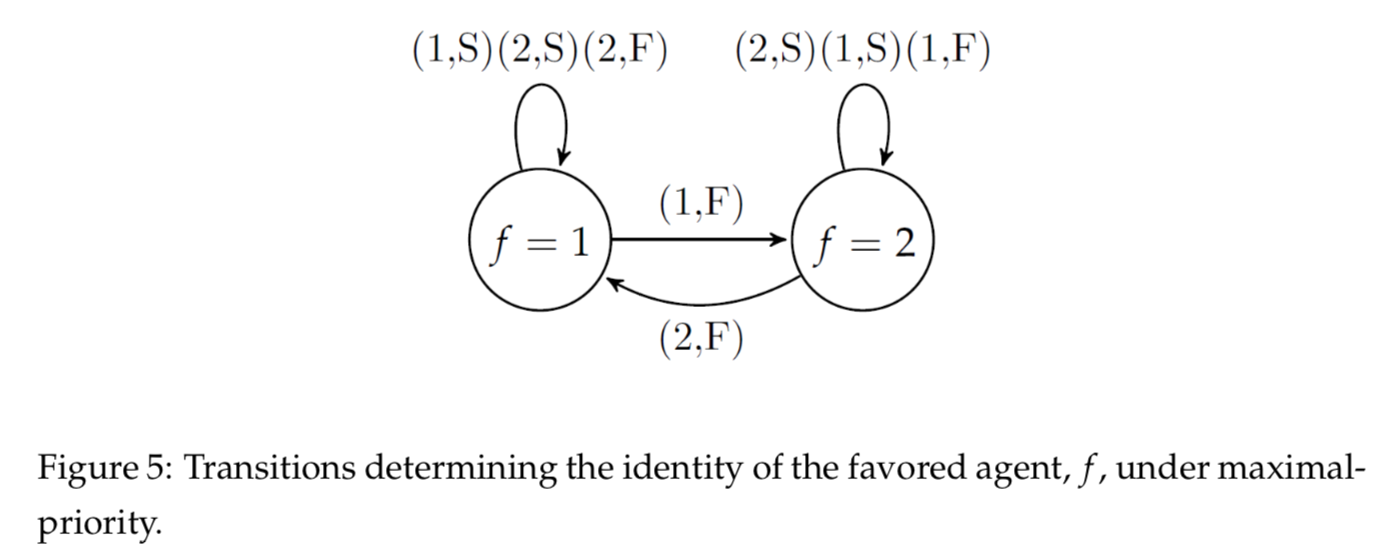
\includegraphics[height=5cm]{image/trans.png}
\end{figure}

\section*{Equivalence between ex-post and performance-based equilibria}
\begin{itemize}
	\item Performance-based: 過去のmessageに依存しない戦略
\end{itemize}


%%%%%%
\newpage
\section*{Preliminaries}

\begin{itemize}
	\item In \S3, we characterize the efficient XPPE payoffs $\mE^*$.
	\item Before entering \S3, we check some basic properties of $\mE^*$: the characterization of $\mE^*$ is reduced to some fixed point problem.
	\item $\mE$: the set of XPPE payoffs.
	\item $\mO:= \text{co} \{(0,0,0), (v^*, \pi v^*, 0), (v^*, 0, \pi v^*)\}$: the set of feasible payoffs. 
	\begin{itemize}
		\item \ocomment{本当に?(0,0,0)は入るのか? $j=0$をモデルに入れるかどうかとも関係?}
		\item $\mO = \{(v_0, v_1, v_2) \in \R^3 \mid v_1 + v_2 = \pi v_0, v \geq 0, v_0 \leq v^*\}$ 
	\end{itemize}
	\item $\mE^* := \{v \in \mE \mid v_1 + v_2 = \pi v^*\}$, where $v^* := \phi (1 - \phi) \underline{\mu} + (1 - \phi (1 - \phi)) \bar{\mu}$
	\item $\mW(V) := \{v \in \R_+^3 \mid v \text{ is decomposable on } V \}$
	\begin{itemize}
		\item \kcomment{Definition of ``decomposability''}
		\item principal's strategy: $\chi(\omega, (m_1, m_2)) = (\chi_1(\omega, (m_1, m_2)), \chi_2(\omega, (m_1, m_2)))\in \{(0,0), (1,0), (0,1)\}$
		\item agent's strategy: $M_{i}(\omega, \theta_i) \in \{0,1\}$
		\item continuation payoffs: $\mV(\omega, m, j, y) \in \R_+^3$, \ocomment{$\mV(\omega, m, j, y) \in \mO$とすべきな気がする.後の証明をみてもそうでないと辻褄が合わない箇所がある.}
		\item policy $\mZ := (\chi, M, \mV)$
		\item \kcomment{(interim) utility functions}
		\begin{itemize}
			\item agent $i \in \{1,2\}$については,ex-post incentive compatibilityを考えるので,他人のtypeが決まっているときについてのutilityを考える.
			$$
			U_i(m_i, \theta_i; \omega, \theta_{-i}, M_{-i}, \chi, \mV) := \dots
			$$
			\item principalについては,普通に期待利得を考える.
			$$U_0(\chi; \omega, M, \mV) := E_\theta[\sum_i \dots]$$
		\end{itemize}
		\item \kcomment{ex-post incentive compatibility (XIC)}: $(\chi, M, \mV)$ satisfies \textit{XIC} if
		\begin{itemize}
			\item agents $i \in \{1,2\}$:
			\[
			\forall (\omega, i, \theta, m_i); \quad  
			U_i(M_i(\omega, \theta_i), \theta_i; \omega, \theta_{-i}, M_{-i}, \chi, \mV) \geq U_i(m_i, \theta_i; \omega, \theta_{-i}, M_{-i}, \chi, \mV)
			\]
			\item principal:
			$$
			\forall (\omega, \tilde{\chi}); \quad
			U_0(\chi; \omega, M, \mV) \geq U_0(\tilde{\chi}; \omega, M, \mV)
			$$
		\end{itemize}
		\item $v$ is \textit{ex-post decomposable (enforceable)} by $\mZ$ on $V \subseteq \R_+^3$ if
		\begin{enumerate}
			\item $\mZ$ satisfies XIC.
			\item $v = \Lambda(\mZ)$, where $\Lambda(\mZ)$ denotes the ex-ante payoff under $\mZ$.
			\item $\forall (\omega, m, j, y); \ \mV(\omega, m, j, y) \in V$
		\end{enumerate}
		\item $v$ is \textit{ex-post E-decomposable} by $\mZ$ on $V \subseteq \R_+^3$ if
		\begin{enumerate}
			\item $v$ is ex-post decomposable by $\mZ$ on $V \subseteq \R_+^3$.
			\item (continuation payoffs attain efficiency) \\
			$\forall (\omega, j, y, \theta); \ \mV_1(\omega, M_1(\theta_1), M_2(\theta_2), j, y) + \mV_2(\omega, M_1(\theta_1), M_2(\theta_2), j, y)= \pi v^*$.
			\item (current allocation is efficient) \\
			(i) The task is allocated to at least one agent, and (ii) if there is a suited agent, the task is allocated to him/her.
		\end{enumerate}
	\end{itemize}
	\item $V \subseteq \R_+^3$: ex-post self-generating $\defi$ $V \subseteq \mW(V)$
\end{itemize}


\begin{lem}[The property of $\mE^*$] \label{lem1}
	\ \\
	(i) $v \in \mathcal{E}^* \implies \text{$v$ is E-decomposed by some $\mZ$ on $\mE^*$}$ \\
	(ii) $\mE^* = \emptyset$, or $\mE^* = \text{co} \{ \hat{v}, \tilde{v} \}$ for some $\hat{v}, \tilde{v} \in \{v \in \R_+^2 \mid v_1 + v_2 = \pi v^*\}$.
\end{lem}
\begin{proof}
	(i) follows from APS self-generation argument. (ii) follows from the existence of public randomization device.
\end{proof}

\begin{itemize}
	\item If $\mE^*$ is nonempty, any vector $v^* \in \mE^*$ can be decomposed by a policy with efficient allocation: there is at least one profile of XPPE strategies that attains $v^*$ as its average payoff.
	\item When is $\mE^*$ empty?
	\item Can we characterize $\mE$, that is, the values of $\hat{v} , \tilde{v}$, in case $\mE \neq \emptyset$.
	\item Fix the primitives $(\delta, \phi, \bar{\mu}, \underline{\mu}, \pi)$.
	\item $\underline{v} := \min \{v \in \R_+ \mid (v^*, v, \pi v^* - v) \in \mE^* \}$. $\bar{v} := \pi v^* - \underline{v}$.
\end{itemize}
\begin{figure}[H]
	\centering
	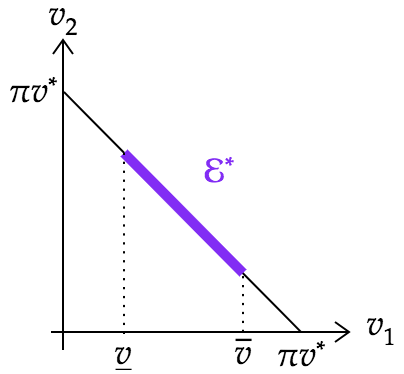
\includegraphics[height=5cm]{image/eff_eq.png}
\end{figure}
\begin{itemize}
	\item $\Psi: [\underline{v}, \frac{1}{2}\pi v^*] \to [\underline{v}, \bar{v}]$. 
\end{itemize}
$$
\Psi(v) := \inf \{ \tilde{v} \in \R_+ \mid 
	(v^*, \tilde{v}, \pi v^* - \tilde{v}) \text{ can be E-decomposable on } \text{co}\{(v^*, v, \pi v^* - v), (v^*, \pi v^* - v, v) \}
\}
$$
\begin{itemize}
	\item $\inf$の中身は$\emptyset$になることもありうる.(その場合$\inf \emptyset = \infty$としておく.)
	\item \ocomment{$n \geq 3$のときも同様な議論ができるか? $\pi v_0 = \sum_i v_i, v \geq 0, v_0 \leq v^*$, $v^*$の定義は要検討}
\end{itemize}

\begin{lem}[The characterization of $\mE$ is reduced to search for the fixed point of $\Psi$.] \ \\
\indent
	If $\mE^* \neq \emptyset$, then $\underline{v}$ is the fixed point of $\Psi$, i.e., $\Psi(\underline{v}) = \underline{v}$.
\end{lem}
\begin{proof}
	Note that $\mE^* = \text{co}\{(v^*, \underline{v}, \pi v^* - \underline{v}), (v^*, \pi v^* - \underline{v}, \underline{v}) \}$ and $\underline{v} \in \mE^*$. Since $\mE^* \subseteq \mW(\mE^*)$ by Lem.\ref{lem1}, $\underline{v}$ is E-decomposable on $\text{co}\{(v^*, \underline{v}, \pi v^* - \underline{v}), (v^*, \pi v^* - \underline{v}, \underline{v}) \}$. Thus, $\Psi(\underline{v}) \leq \underline{v}$. 
	
	We want to show that $\Psi(\underline{v}) = \underline{v}$. Suppose toward contradiction that $\Psi(\underline{v}) < \underline{v}$.
	Then, there exists $\tilde{v}$ such that $\Psi(\underline{v}) < \tilde{v} < \underline{v}$.
	By definition of $\Psi$, $(v^*, \tilde{v}, \pi v^* - \tilde{v})$ can be E-decomposed on $\text{co} \{(v^*, \underline{v}, \pi v^* - \underline{v}), (v^*, \pi v^* - \underline{v}, \underline{v}) \} = \mE^* \subseteq \mE$.
	In particular, $(v^*, \tilde{v}, \pi v^* - \tilde{v}) \in \mW(\mE) = \mE$. Note that, since $\tilde{v} + (\pi v^* - \tilde{v}) = \pi v^*$, if $(v^*, \tilde{v}, \pi v^* - \tilde{v}) \in \mE$, then $\tilde{v} \in \mE^*$. By definition of $\underline{v}$, $\tilde{v} \notin \mE^*$, and thus $\tilde{v} \notin \mE$. A contradiction.	
\end{proof}


\subsection*{Technical Problems}
\begin{itemize}
	\item DP with uncertainty. (One-shot deviation principles with uncertainty)
	\item Self-generation (compactness of the set of equilibrium payoffs)
	\item public randomization (convexity of the set of equilibrium payoffs)
\end{itemize}

\section*{Proofs for Section 3}
\begin{itemize}
	\item Characterize the set of efficient XPPE payoffs $\mathcal{E}^*$.
	\item Note that if $v \in \mO$ is E-decomposed by $\mZ := (\chi, M, \mV)$ on $V \subseteq \mO$, then the principal has no incentive to deviate from $\chi$: By the definition of E-decomposition, both present and continuation payoffs of the principal are maximized.
\end{itemize}
\begin{lem}
\ocomment{元論文のlemmaの主張はよくわからない.Revelation Principleのようなもの?}\\
Suppose a policy $\mZ' := (\chi', M', \mV')$ E-decompose $v \in \mO$ on $V \subseteq \mO$. Then, we can construct $\mZ:=(\chi, M, \mV)$ that decomposes $v$ on $V$ with the following properties:
\begin{itemize}
	\item Both agents tell their type truthfully: $\forall i \forall (\omega, \theta_i); \ M_i(\omega, \theta_i) = 1 \text{ iff } (\omega, \theta_i) \in \{(A, \alpha), (B, \beta)\}$
%	\item Allocations are determined as follows: for all $\omega$,
\end{itemize}
%\begin{enumerate}
%	\item $(m_i, m_{-i}) = (1, 0) \implies \chi_i^\omega(m) = 1$
%	\item $\exists i; [(m_i, m_{-i}) = (1, 1) \implies \chi_i^\omega(m) = 1], \ [(m_i, m_{-i}) = (0, 0) \implies \chi_{-i}^\omega(m) = 1] $ \\
%		($-i$のmessageは無視される.)
%\end{enumerate}	
\end{lem}
\begin{proof}(\ocomment{Incomplete})
	Suppose $\mZ' := (\chi', M', \mV')$ E-decompose $v \in \mO$ on $V \subseteq \mO$.
	
	First, we show at least one agent need to change his message according to his own type under $\mZ'$:
	$$
	\forall \omega \exists i; \ M_i(\omega, \alpha) \neq M_i(\omega, \beta)
	$$
	Suppose toward contradiction that there is some $\omega$ such that both agents pool their information, i.e., $\exists \omega \ \forall i; M'_i(\omega, \alpha) = M'_i(\omega, \beta)$, then this leads to a contradiction: For such $\omega$, we can show that $U_0^\omega(\chi', M', \mV') = v_0 < v^*$, which contradicts the fact that $v$ is E-decomposed by $\mZ'$.
	
	Next, we show that we can construct $\mZ$ that E-decomposes $v$ on $V$ and $M_i(\omega, \theta_i)$ is truth-telling for all $i$. Fix $\omega$.
	\paragraph{Case (i): In case $\forall i; \ M_i(\omega, \alpha) \neq M_i(\omega, \beta)$:}
	By relabeling, we can construct $\mZ$.
	\paragraph{Case (ii): In case $\exists i; M_i(\omega, \alpha) = M_i(\omega, \beta)$:} Assume without loss of generality, $i:=1$. If agent 1 is not truth-telling, then relabeling is needed. As for agent 2, assume w.l.o.g that $M_2(\omega, \theta_2) \equiv 1$. Consider the following modification:
	\begin{align*}
		\chi_i^{\omega}(m_1, m_2) &:= \chi_i^{\omega'}(m_1, 1) \\
		\mV_i^{\omega}((m_1, m_2), j, y) &:= \mV_i^{\omega'}((m_1, 1), j, y)
	\end{align*}
	
	
%	Next, we show that without loss of generality we can ignore the case where there exists $\omega$ for which one agent pools his information: If $\exists \omega \exists i; \ M'_i(\omega, \alpha) = M'_i(\omega, \beta)$, then we can construct another policy $\mZ$ that E-decomposes $v$ on $V$.
	
%	Suppose $\mZ' := (\chi', M', \mV')$ E-decompose $v$ on $V$, and $\exists \omega \exists i; \ M'_i(\omega, \alpha) = M'_i(\omega, \beta)$.
%	If this is the case, define $\chi(\omega, \cdot)$ that ignores $i's$ message. Then, it is also incentive compatible for $i$ to tell his type truthfully, i.e., define $M$
\end{proof}

\begin{itemize}
	\item XIC conditions for agents' truth-telling can be represented as a system of linear equations.
	\item \kcomment{(IC1) - (IC6)}
	\item Agent 1's ex-ante payoff $\Lambda_1$ can also be explicitly written.
\end{itemize}

\begin{lem}\label{revelation}
Suppose $\mE^* \neq \emptyset$.	Then, for any $v \in [\underline{v}, \frac{1}{2}\pi v^*]$,
$$
\Psi(v) = 
\left[
\begin{array}{ccc}
	 \displaystyle{\min_{\chi, \mV}} & \Lambda_1  &  \\
	 \text{ s.t.}      & \text{XIC: (IC1)-(IC6)} \\
	 & \chi_1^\omega(m) + \chi_2^\omega(m) = 1 \\
	 & (m_i, m_{-i}) = (1,0) \implies \chi_i^\omega(m) = 1 \\
	 & \mV_i^\omega(m,j,y) \in [v, \pi v - v^*] \\
	 & \mV_1^\omega(m,j,y) + \mV_2^\omega(m,j,y) = \pi v^* \\
	 & \forall \omega \in \{A, B\}, m \in \{0,1\}^2, i,j \in \{1,2\}, y \in \{S, F\}
\end{array}
\right.
$$
\end{lem}
\begin{proof}
	By Lem.\ref{revelation}.
\end{proof}

\begin{itemize}
	\item 上の問題を頑張って解く.\ocomment{一応頑張って式は追ってみたが,キチンと理解できていない.}
	\item \ocomment{線形計画問題を頑張って解いているとだけみなせる・・・?}
\end{itemize}

\begin{lem}
	$$
	\mE^* \neq \emptyset \equi \phi(1 - \phi) \geq \frac{\underline{\mu}(1 - \delta \bar{\mu})}{\delta (\bar{\mu} - \underline{\mu})(1 - \underline{\mu})}
	$$
\end{lem}

\section*{Proofs for Section 4}
\subsection*{Prop.5}
straight forward. XIC conditions and the definition of $v^f$ and $v^{-f}$.


\section*{なにができそう?}
\begin{itemize}
	\item $n \geq 3$で何が起こるか?
	\begin{itemize}
		\item 効率的な均衡利得の特徴付けは,self-generationの議論のあとはただの線形計画問題な気がするので,$n \geq 3$にしても拡張できそうな気もする.(Lem.10のproofをもう少しきちんと理解する必要)
		\item maximal-priorityは人数が増えるとどうなるのか?
	\end{itemize}
	\item principalがコミットできるとするとどうなるのか?(効率性が達成しやすくなる?)
	\item first-bestが達成可能でない場合に何が起きているかをもうちょっと詳しくみる?
	\item learning -- 片方についてのみ$\phi^i$が未知とかにするとどうなる?
\end{itemize}

\end{document}